%%%%%%%%%%%%%%%%%% ATLAS

\section{The ATLAS Experiment}
\label{sed:cern:atlas}

ATLAS (A Toroidal LHC ApparatuS)\cite{atlas:atlas} is the largest of the LHC detectors: as it is shown in Fig. \ref{fig:atlas:atlas} it measures 44 meters in length and 25 meters in height, and its weights is about 700 tons. To be fully functional in the LHC environment,  ATLAS needs to be fast as it needs to be able to resolve the collisions resulting from consecutive bunches (which are interspaced by 25 ns) and radiation resistant. 

\begin{figure}[ht]
\centering
\subfigure{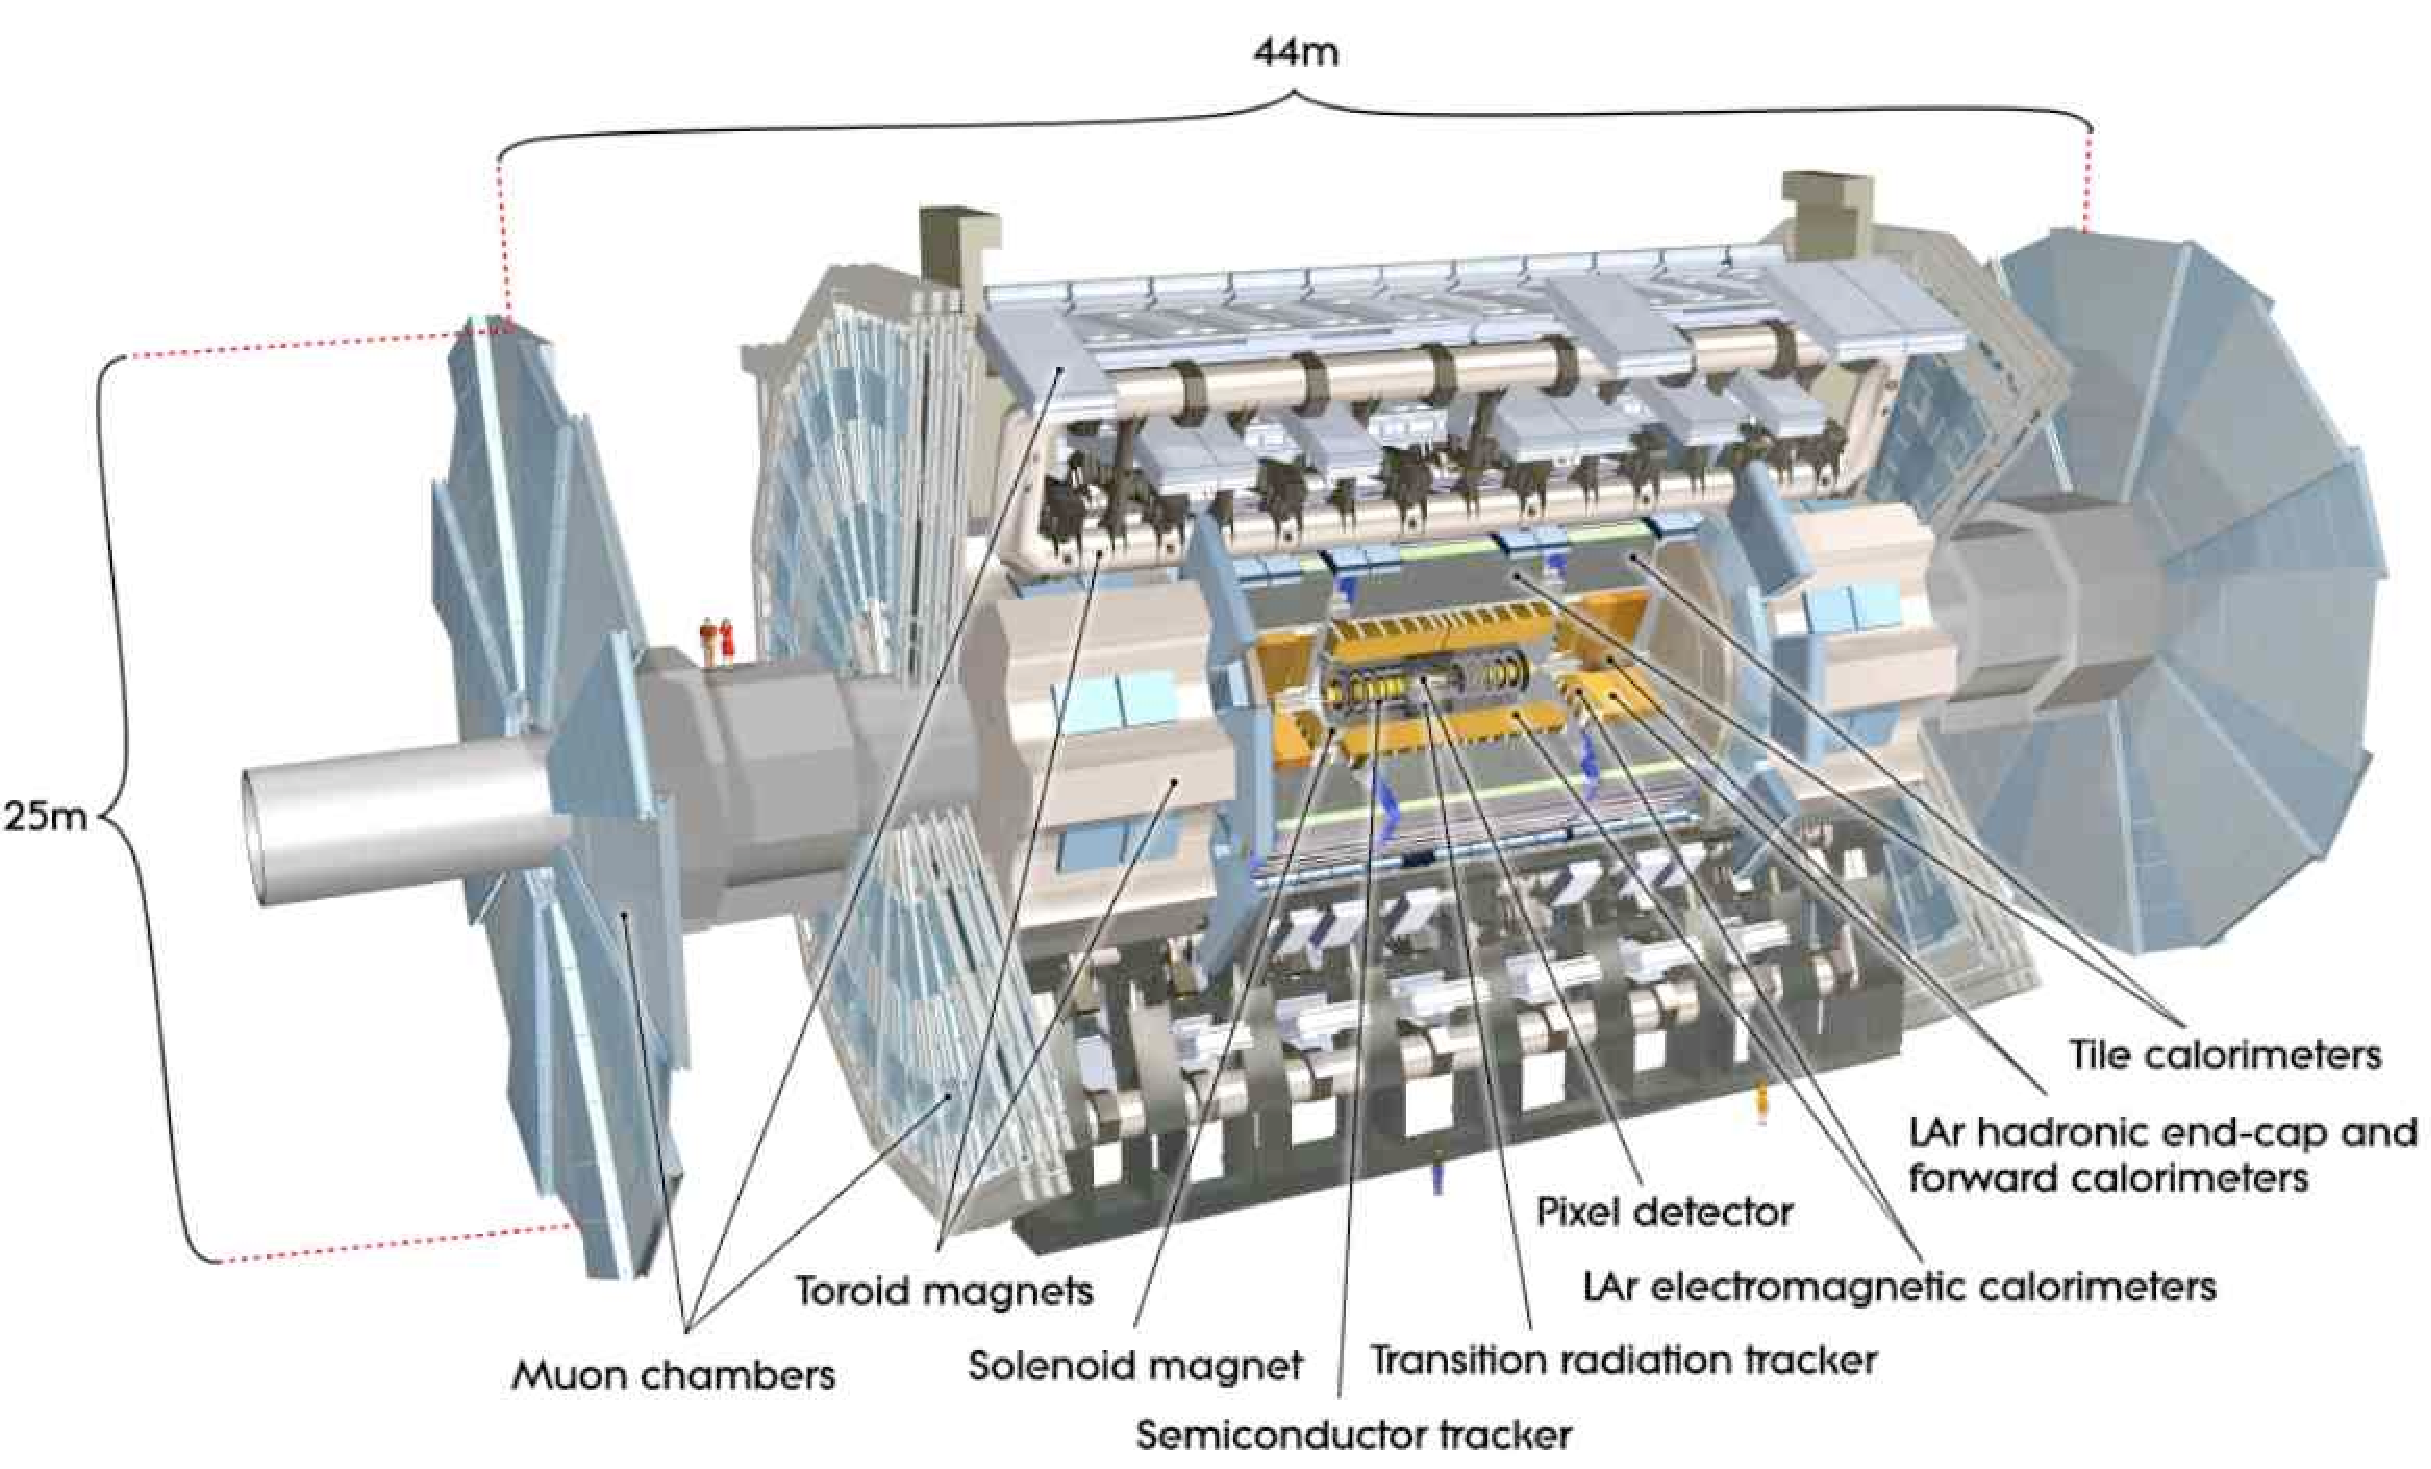
\includegraphics[width=0.85\textwidth]{figures/atlas/atlas}}
\caption{Computer-generated image of the ATLAS inner detector. Figure from Ref. \cite{atlas:atlas}}
\label{fig:atlas:atlas}
\end{figure}

The ATLAS physics program covers a large variety of topics: 
\begin{itemize}
\item Standard Model processes can be measured at the LHC at energies never reached before, and being sensitive to them is essential both to provide accurate measurements and to use them as candles to calibrate the detector. 
\item The discovery of the Higgs boson was one of the main goals of the LHC, and after its observation in 2013 the focus moved on measuring its properties. 
\item Top quarks are produced in large amount at the LHC, and the study of the properties of this particle can both probe the SM and set limits on BSM theories.
\item The LHC offers an incredible opportunity to discover BSM physics, and ATLAS needs to be ready to identify its signs.
\item Despite the ALICE detector is specifically designed to study heavy-ion collisions, ATLAS also carries out an heavy-ion program.
\end{itemize}

To cope with the wide range of types and energies (from few GeV to several TeV) of the particles that need to be identified, ATLAS relies on a sequence of subdetectors nested in a cylindrical geometry, that follow the general schema discussed in Section \ref{sec:detectors:identification}: close to the interaction point we find the inner detector (ID), embedded in a magnetic field of 2 T. The following layers are the electromagnetic and the hadronic calorimeters (ECal and HCal), and the outermost part is occupied by the muon system. All of these components are described in the next sections.

\subsection{Coordinate System}

ATLAS uses a right-handed coordinate system, with its origin at the nominal interaction point. The $z$-axis follows the beam direction, while in the transverse plane the $y$-axis points upward and the $x$axis toward the LHC center. Positive and negative values of the $z$-axis identify respectively the A-side and the C-side of the detector. When spherical coordinates are used, the \textit{azimuthal angle} $\phi$ is defined starting from the $x$-axis, and ranges between $-\pi$ and $\pi$; the \textit{polar angle} $\theta$ is defined starting from the $z$-axis and takes values between $0$ and $\pi$. Often the polar angle is substituted by the \textit{pseudorapidity}: 
 
\begin{equation}
\label{eq:cern:eta}
\eta = - \ln \tan \frac{\theta}{2}
\end{equation}

which, in the limit of massless particles, is equivalent to the \textit{rapidity}:

\begin{equation}
\label{eq:cern:y}
y = \frac{1}{2} \ln \frac{E + p_z}{E - p_z} \; ,
\end{equation}

where $E$ is the energy of the particle and $p_z$ its momentum projected on the $z$-axis. The $\eta$-$\phi$ plane is used to define the angular separation of two objects in the detector:

\begin{equation}
\label{eq:cern:dR}
\Delta R = \sqrt{ \Delta \phi^2 + \Delta \eta^2  } \; .
\end{equation}

Since protons are composite particles, and the hard scattering happens between its constituents, the longitudinal momentum of the partons is unknown. It is therefore useful to define the \textit{transverse momentum} as the projection of the momentum on the ($x$,$y$) plane: 

\begin{equation}
\label{eq:cern:pt}
p_T = \sqrt{p_x^2 + p_y^2} \; ,
\end{equation}

where $p_{x(y)}$ are the projection of the momentum along the $x$-($y$-)axis.




\subsection{Magnet System}

\label{sec:cern:atlasmagnets}
\begin{figure}[ht]
\centering
\subfigure{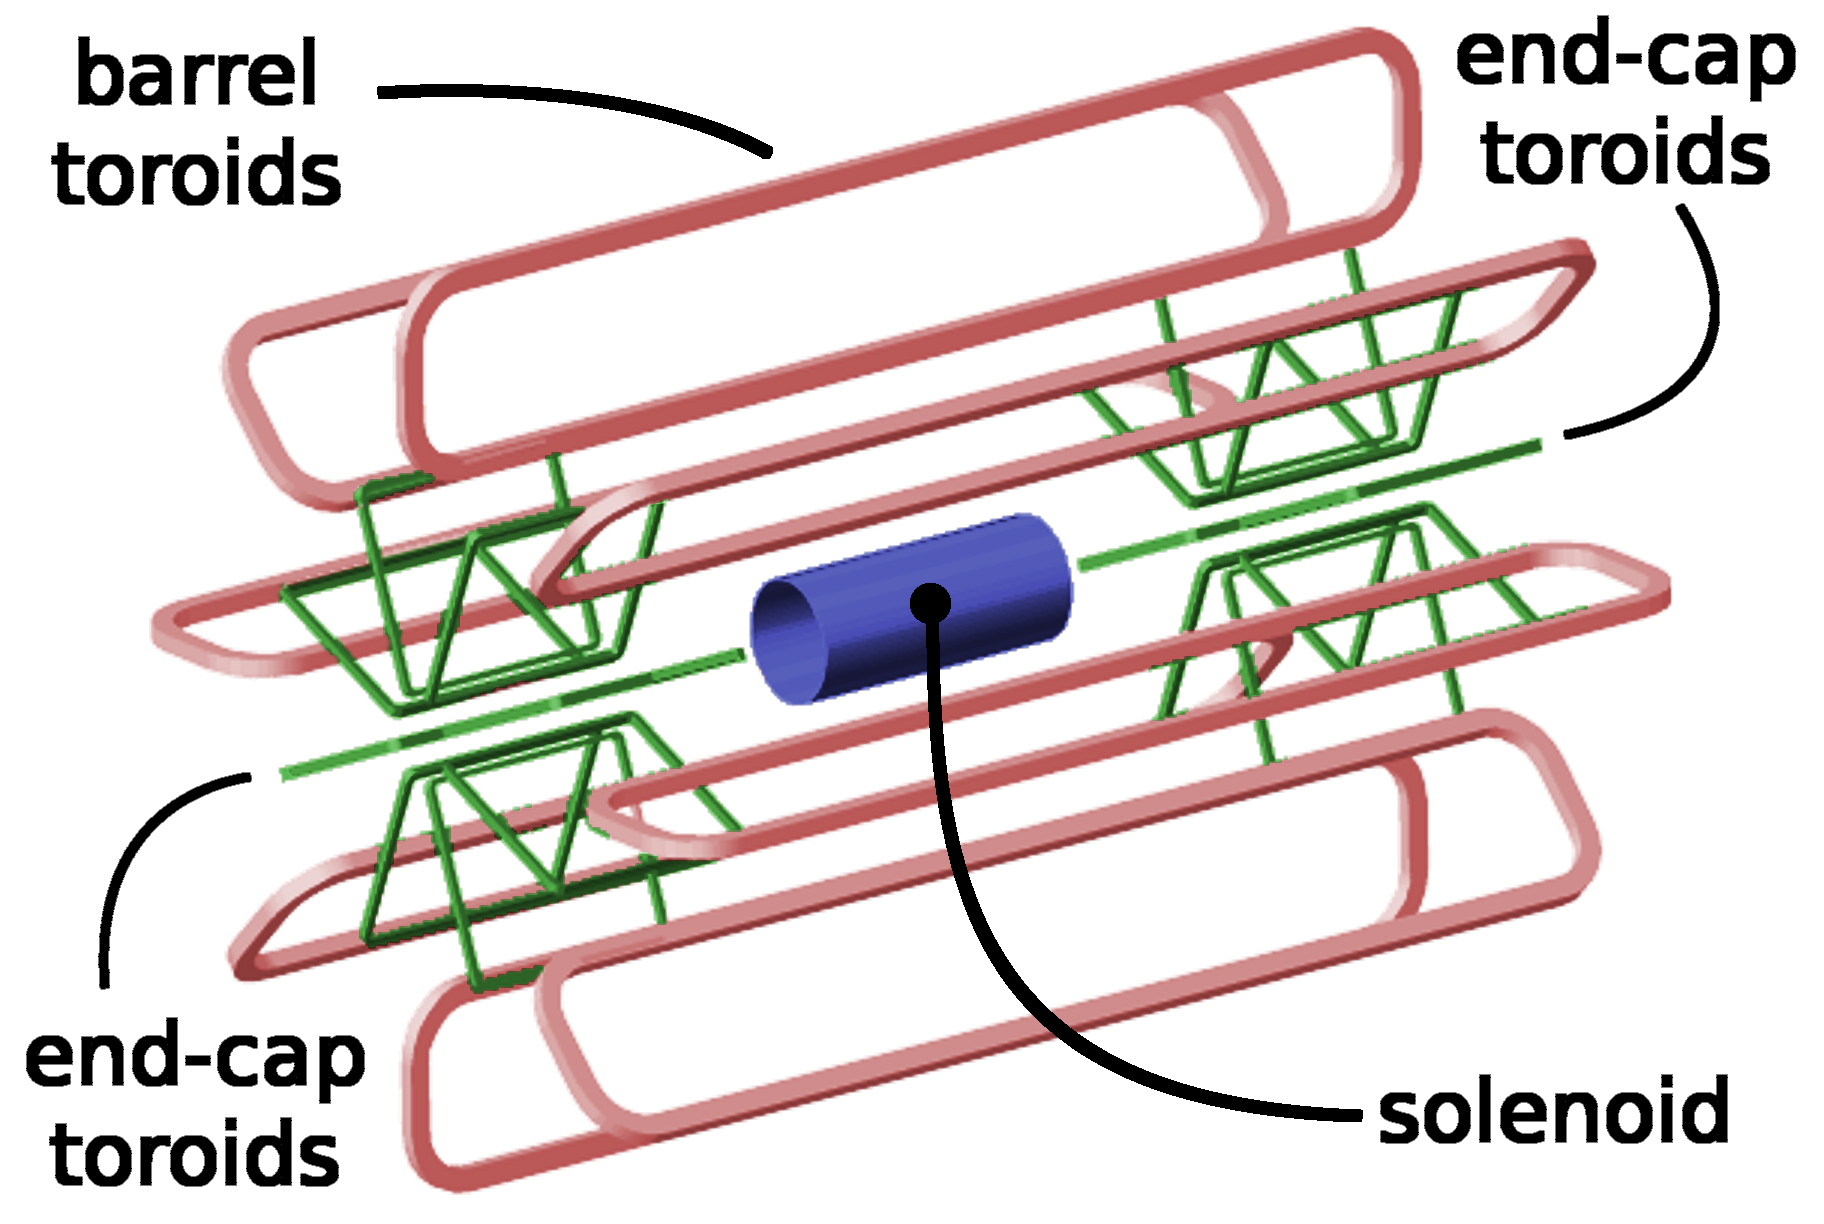
\includegraphics[width=0.35\textwidth]{figures/atlas/magnets}}
\caption{Layout of the ATLAS magnet system. Figure from Ref. \cite{Goodson}}
\label{fig:atlas:magnet}
\end{figure}



\subsubsection*{Solenoid}

\subsubsection*{Toroids}



\subsection{Inner Detector}

\begin{figure}[ht]
\centering
\subfigure{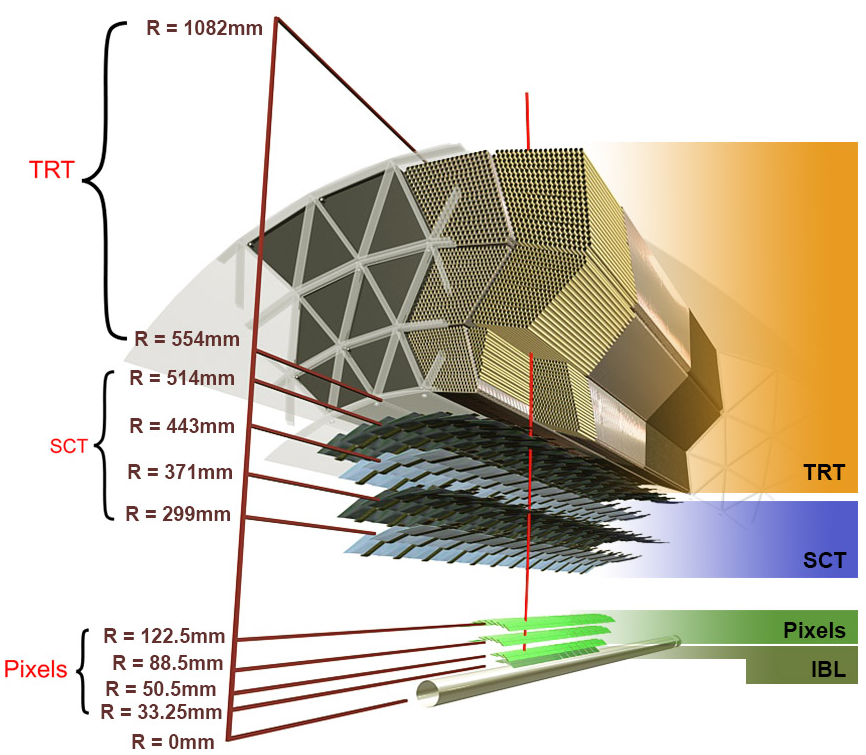
\includegraphics[width=0.65\textwidth]{figures/atlas/inner_detector}}
\caption{Layout of the ATLAS inner detector. Figure from Ref. \cite{Potamianos:2016ptf}}
\label{fig:atlas:id}
\end{figure}


\subsubsection*{Pixel Detector}


\subsubsection*{Semi-Conductor Tracker}


\subsubsection*{Transition Radiation Tracker}



\subsection{Calorimeters}

\begin{figure}[ht]
\centering
\subfigure{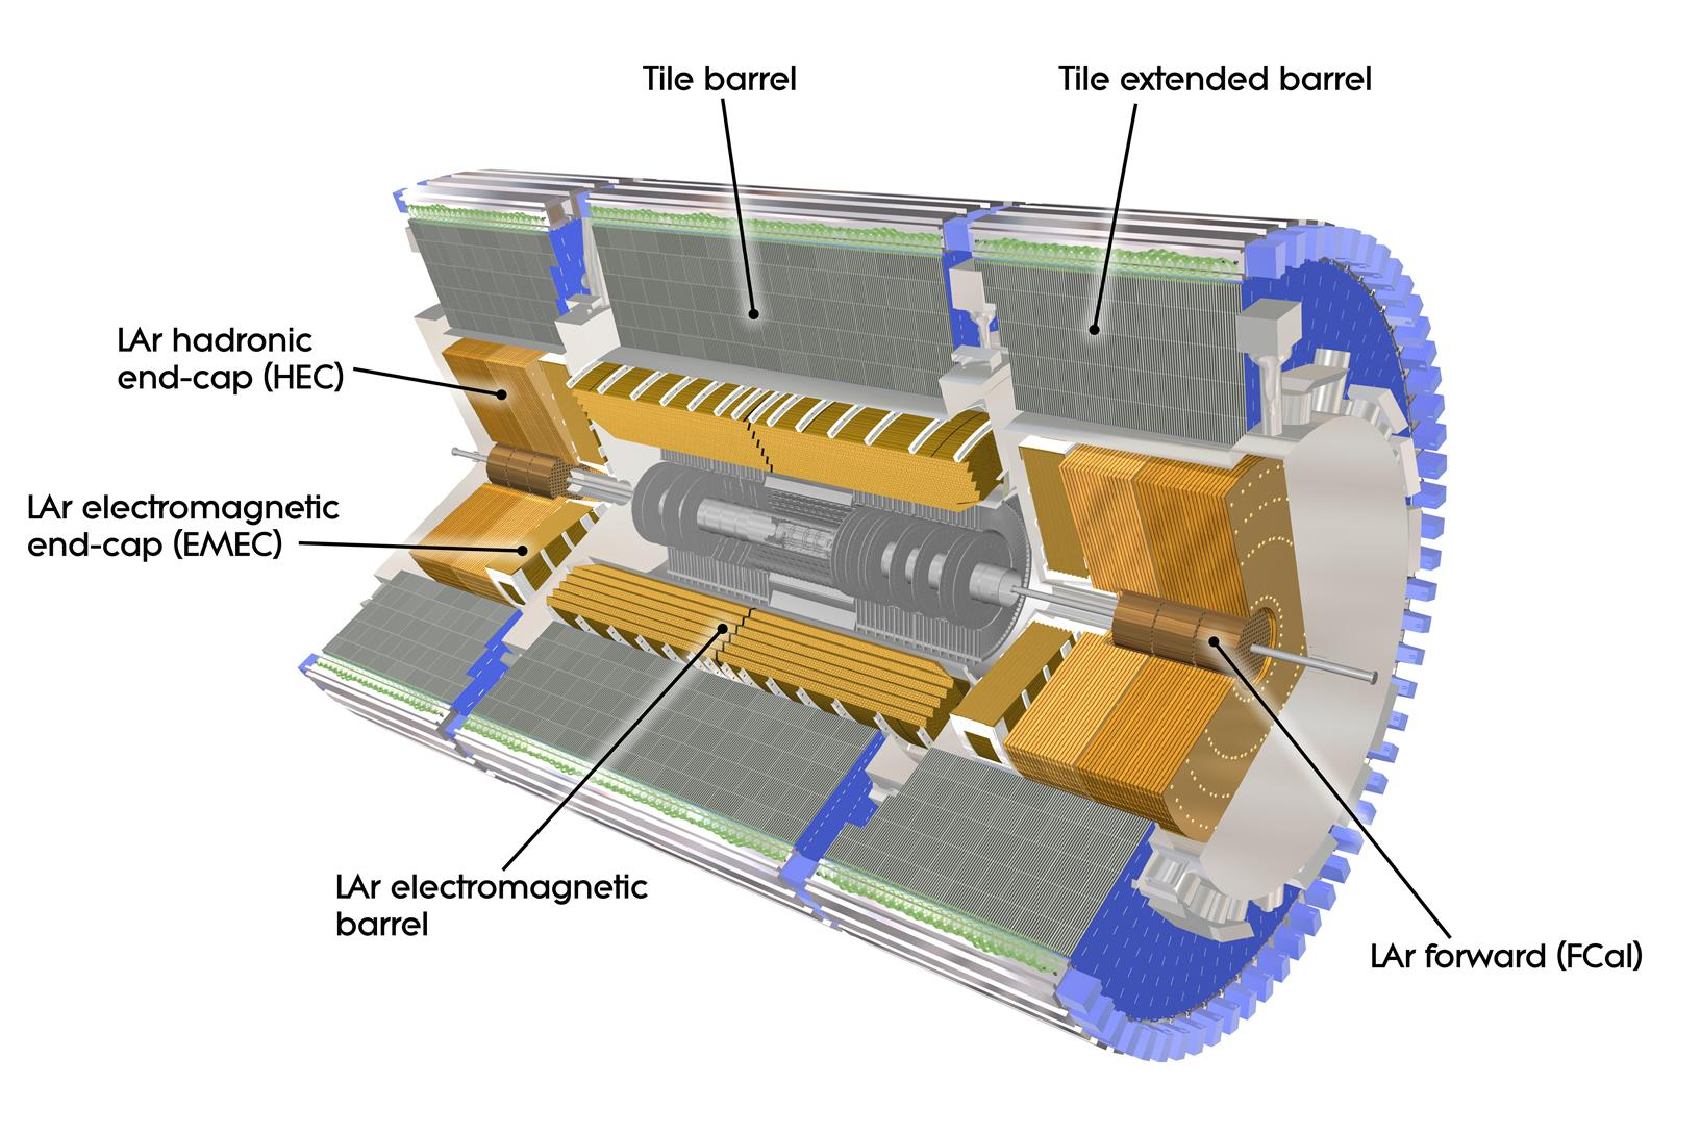
\includegraphics[width=0.75\textwidth]{figures/atlas/calorimeters}}
\caption{Layout of the ATLAS calorimeter system. Figure from Ref. \cite{atlas:atlas}}
\label{fig:atlas:calo}
\end{figure}

\subsubsection*{Electromagnetic Calorimeter}


\subsubsection*{Hadronic Calorimeter}


\subsubsection*{Forward Calorimeter}


\subsection{Muon Spectrometer}

\begin{figure}[ht]
\centering
\subfigure{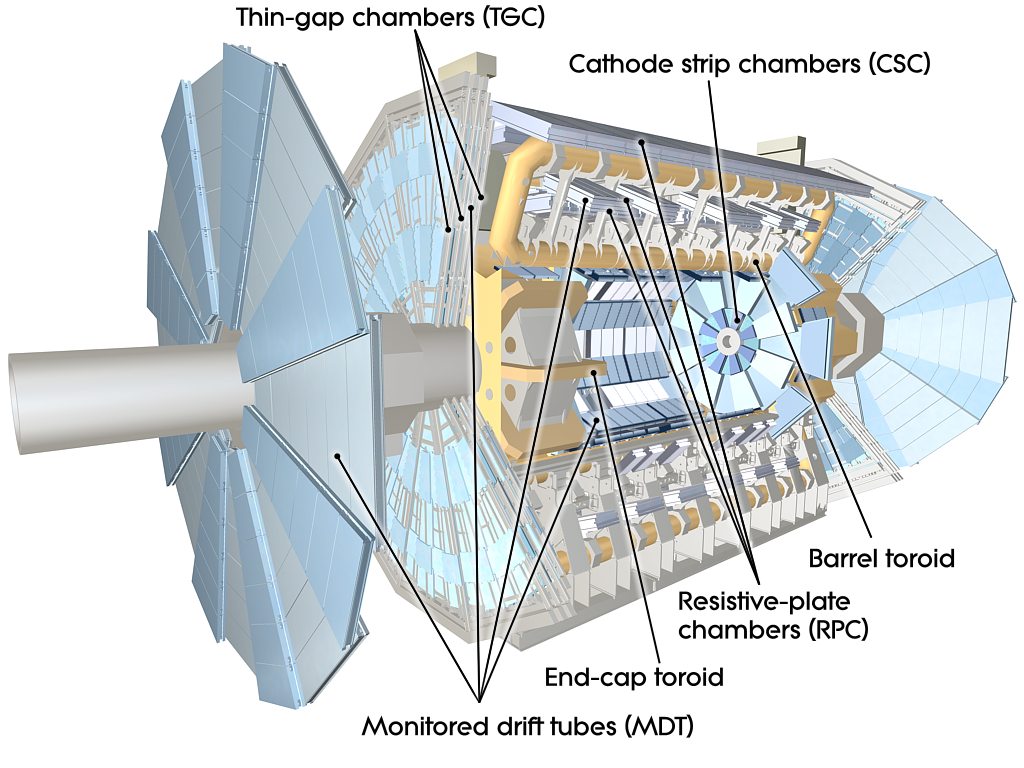
\includegraphics[width=0.65\textwidth]{figures/atlas/muon}}
\caption{Layout of the ATLAS muon system. Figure from Ref. \cite{atlas:atlas}}
\label{fig:atlas:muon}
\end{figure}

\subsection{Luminosity Detectors}

\subsection{Trigger System}
\label{sec:cern:trigger}

\subsection{ATLAS Performance Summary}

